\documentclass[reqno, 12pt]{article}
\usepackage{enumerate}
\usepackage{amsmath}
\usepackage{scrextend}
\usepackage{bm}
\usepackage{algorithm}
\usepackage{algpseudocode}
\usepackage{graphicx}
\usepackage{enumitem}
\usepackage{tcolorbox}
\usepackage[headheight=12pt,textwidth=7in,top=1in, bottom=1in]{geometry}
\usepackage{listings}
\usepackage{cancel}
\usepackage{color} %red, green, blue, yellow, cyan, magenta, black, white
\definecolor{mygreen}{RGB}{28,172,0} % color values Red, Green, Blue
\definecolor{mylilas}{RGB}{170,55,241}
\usepackage{dirtree}

\usepackage[]{xcolor}
\definecolor{lightblue}{rgb}{0.63, 0.74, 0.78}
\definecolor{seagreen}{rgb}{0.18, 0.42, 0.41}
\definecolor{orange}{rgb}{0.85, 0.55, 0.13}
\definecolor{silver}{rgb}{0.69, 0.67, 0.66}
\definecolor{rust}{rgb}{0.72, 0.26, 0.06}
\definecolor{purp}{RGB}{68, 14, 156}

\colorlet{lightrust}{rust!50!white}
\colorlet{lightorange}{orange!25!white}
\colorlet{lightlightblue}{lightblue}
\colorlet{lightsilver}{silver!30!white}
\colorlet{darkorange}{orange!75!black}
\colorlet{darksilver}{silver!65!black}
\colorlet{darklightblue}{lightblue!65!black}
\colorlet{darkrust}{rust!85!black}
\colorlet{darkseagreen}{seagreen!85!black}

\usepackage{hyperref}
\hypersetup{
  colorlinks=true,
}

\hypersetup{
  linkcolor=darkrust,
  citecolor=seagreen,
  urlcolor=darkrust,
  pdfauthor=author,
}

\usepackage{cleveref}

%some custom commands you may find useful
\usepackage{xparse}
\DeclareDocumentCommand{\diff}{O{} m}{
	\frac{\mathrm{d} #1}{\mathrm{d}#2}
}
\DeclareDocumentCommand{\difftwo}{O{} m}{
	\frac{\mathrm{d}^2 #1}{\mathrm{d}#2^2}
}
\DeclareDocumentCommand{\pdiff}{O{} m}{
	\frac{\partial #1}{\partial #2}
}
\DeclareDocumentCommand{\pdifftwo}{O{} m}{
	\frac{\partial^{2} #1}{\partial #2^{2}}
}
\DeclareDocumentCommand{\integral}{O{} O{} m O{x}}{
	\int_{#1}^{#2} #3\ \mathrm{d}#4
}
\DeclareDocumentCommand{\sp}{}{
	\qquad \qquad \qquad }{
}
\NewDocumentEnvironment{solution}{}{
	\begin{addmargin}[2em]{0pt}
	}{\end{addmargin} \vskip0.25cm
}

\newenvironment{sysmatrix}[1]
{\left(\begin{array}{@{}#1@{}}}
	{\end{array}\right)}
\newcommand{\ro}[1]{%
	\xrightarrow{\mathmakebox[\rowidth]{#1}}%
}
\newlength{\rowidth}% row operation width
\AtBeginDocument{\setlength{\rowidth}{3em}}

\def\name{Ben Wilfong} %your name goes here
\def\ID{bwilfong3} %your cm goes here

%these packages create the footer and page numbering
\usepackage{fancyhdr}
\usepackage{lastpage}
\pagestyle{fancy}
\lhead{\name}
%%%%%%%%%%%%%%%%%%%%%%%%%%%%%%%%
\chead{ME 7751 Homework \#1}
%%%%%%%%%%%%%%%%%%%%%%%%%%%%%%%%
\rhead{Username: \ID}
\fancyfoot[C]{\footnotesize Page \thepage\ of \pageref{LastPage}}
\fancypagestyle{firststyle}
{ \renewcommand{\headrulewidth}{0pt}%
	\fancyhf{}%
	\fancyfoot[C]{\footnotesize Page \thepage\ of \pageref{LastPage}}
}

\lstset{frame=tb,
  language=[90]Fortran,
  aboveskip=3mm,
  belowskip=3mm,
  showstringspaces=false,
  columns=flexible,
  basicstyle={\footnotesize\ttfamily},
  numbers=none,
  numberstyle=\tiny\color{gray},
  keywordstyle=\color{darklightblue},
  commentstyle=\color{seagreen},
  stringstyle=\color{darkrust},
  breaklines=true,
  breakatwhitespace=true,
  tabsize=3,
}

\begin{document}
	\noindent
    \thispagestyle{firststyle}
	%\begin{tabular}{l}
		%{\LARGE \textbf{ME 7751: Intro to CFD} }\\
		%%%%%%%%%%%%%%%%%%%%%%%%%%
		%{\Large Homework Set \#1}
		%%%%%%%%%%%%%%%%%%%%%%%%%%
	%\end{tabular} \hfill \begin{tabular}{r}
		%\name \\
		%Username: \ID
	%\end{tabular}
	%\noindent\makebox[\linewidth]{\rule{\textwidth}{1pt}}
    \begin{center}
        \LARGE{\textbf{Solution of the 1D steady transport equation with the finite difference method}} \\
        \Large{September 16$^{th}$, 2024} \\
        \large{Ben Wilfong}
    \end{center}
    \section*{Files}
    \dirtree{%
        .1 HW1\_root.
         .2 CMakeLists.txt.
         .2 README.md.
         .2 homework.pdf.
         .2 main.inp.
         .2 make.sh.
         .2 src.
         .3 m\_global\_parameters.f90.
         .3 m\_helpers.f90.
         .3 m\_linear\_algebra.f90.
         .3 p\_main.f90.
         .2 plots.
         .3 outputB10.csv.
         .3 outputB20.csv.
         .3 outputB30.csv.
         .3 outputB40.csv.
         .3 outputB50.csv.
         .3 outputC1.csv.
         .3 outputC2.csv.
         .3 outputC3.csv.
         .3 plots.m.
    }
    \section*{Compiling}
    This code can be compiled in a terminal by running \texttt{chmod u+x ./mfc.sh} followed by \texttt{./mfc.sh} in the \texttt{HW1\_root/} directory.
    This will compile and link the source code in the \texttt{src/} directory and create an executable called \texttt{main} in the \texttt{HW1\_root/} directory.
    \section*{Running}
    The problem parameters are defined in the namelist file \texttt{main.inp} in \texttt{HW1\_root/}.
    The input parameters are:
    \begin{itemize}
        \setlength\itemsep{-0.25em}
        \item gamma0: The coefficient for the zero degree term in the polynomial defining gamma
        \item gamma1: The coefficient for the first degree term in the polynomial defining gamma
        \item L: The length of the domain
        \item N: The number of cells to use
        \item Q0: The coefficient for the zero degree term in the polynomial defining Q
        \item Q1: The coefficient for the first degree term in the polynomial defining Q
        \item U: The convective velocity
        \item tol: Convergence tolerance for nonlinear problems
        \item bench: Toggles benchmarking mode. When true, the code is ran $1\times 10^6$ times and the average runtime is output.
    \end{itemize}
    Once the input parameters are set, the code is ran with \texttt{./main}.
    After execution, the solution is writen to \texttt{HW1\_root/output.csv} with the first column holding the x coordinates and the second column holding the solution.
    Additionally, the following will be written to the terminal:
    \begin{verbatim}
     Solving the 1D Steady Transport Equation with:
     gamma0:   0.10000000000000001
     gamma1:   0.10000000000000001
     U:    0.0000000000000000
     Q0:    0.0000000000000000
     Q1:    0.0000000000000000
     N:           20
     Execution time:    4.99999987E-05  s
     Iterations:           12
    \end{verbatim}
    \vspace{-0.25in}
    This serves as a sanity check for the problem parameters and provides the runtime and number of iterations to convergence.
    Plots are created by running \texttt{plots.m} from the \texttt{root/plots/} directory.
    \newpage

    \section*{Part A - Numerical Method}
    \noindent The one dimensional steady state transport equation
    \begin{equation*}
        U\pdiff[\phi]{x} = \pdiff{x}\left(\Gamma \pdiff[\phi]{x}\right) + Q
    \end{equation*}
    can be discretized with central differences as
    \begin{equation}
        U\frac{\phi_{i + 1} - \phi_{i - 1}}{2\Delta x} - \underbrace{\frac{\left(\Gamma\pdiff[\phi]{x}\right)_{i + 1/2} - \left(\Gamma \pdiff[\phi]{x}\right)_{i - 1/2}}{\Delta x}}_{b} = Q_i.
    \label{eqn:a}
    \end{equation}
    The first derivatives in the numerator of $b$ can be written as
    \begin{equation}
        \left(\Gamma\pdiff[\phi]{x}\right)_{i + 1/2} = \Gamma_{i + 1/2}\frac{\phi_{i + 1} - \phi_{i}}{\Delta x}\quad \text{ and  }\quad \left(\Gamma\pdiff[\phi]{x}\right)_{i - 1/2} = \Gamma_{i - 1/2}\frac{\phi_{i} - \phi_{i-1}}{\Delta x}.
    \label{eqn:b}
    \end{equation}
    Substituting \cref{eqn:b} into \cref{eqn:a} and rearanging gives
    \begin{align}
    U\frac{\phi_{i + 1} - \phi_{i - 1}}{2\Delta x} -
    \frac{\Gamma_{i + 1/2}\frac{\phi_{i + 1} - \phi_{i}}{\Delta x} - \Gamma_{i - 1/2}\frac{\phi_{i} - \phi_{i - 1}}{\Delta x}}{\Delta x} & = Q_i \notag \\
    U\frac{\phi_{i + 1} - \phi_{i - 1}}{2\Delta x} -
    \frac{\Gamma_{i + 1/2}\phi_{i + 1} - (\Gamma_{i + 1/2} + \Gamma_{i - 1/2})\phi_{i} + \Gamma_{i - 1/2}\phi_{i -1}}{\left(\Delta x\right)^2} &= Q_i \notag \\
    \left(\frac{U}{2\Delta x} - \frac{\Gamma_{i + 1/2}}{(\Delta x)^2}\right)\phi_{i + 1} +
    \left(\frac{\Gamma_{i + 1/2} + \Gamma_{i - 1/2}}{(\Delta x)^2}\right)\phi_i -
    \left(\frac{U}{2\Delta x} + \frac{\Gamma_{i - 1/2}}{(\Delta x)^2}\right)\phi_{i - 1} &= Q_i \label{eqn:c}.
    \end{align}
    \Cref{eqn:c} can be cast as the system of linear equations
    \begin{equation*}
        \underbrace{\begin{bmatrix}
        1 \\
        -\left(\frac{U}{2\Delta x} + \frac{\Gamma_{1/2}}{(\Delta x)^2}\right) & \frac{\Gamma_{3/2}+\Gamma_{1/2}}{(\Delta x)^2} & \frac{U}{2\Delta x} - \frac{\Gamma_{3/2}}{(\Delta x)^2} \\
        \ddots & \ddots & \ddots \\
        & -\left(\frac{U}{2\Delta x} + \frac{\Gamma_{N - 3/2}}{(\Delta x)^2}\right) & \frac{\Gamma_{N - 1/2}+\Gamma_{N - 3/2}}{(\Delta x)^2} & \frac{U}{2\Delta x} - \frac{\Gamma_{i -1/2}}{(\Delta x)^2} \\
        &&& 1
\end{bmatrix}}_{\mathrm{\bm{A}}}
\underbrace{\begin{pmatrix} \phi_{0} \\ \phi_{1} \\ \vdots \\ \phi_{N-1} \\ \phi_{N} \end{pmatrix}}_{\Phi}
        =
        \underbrace{\begin{pmatrix} 1 \\ Q_1 \\ \vdots \\ Q_{N-1} \\ 0 \end{pmatrix}}_{b}
    \end{equation*}
    for a discretization at $\{x_0,\ x_1,\ \dots \, x_N\} = \{0,\ \Delta x,\ 2\Delta x,\dots,\ N\Delta x$\}.
    The boundary conditions are given by $\phi_{-1/2} = 1$ and $\phi_{N + 1/2} = 0$. \\~\\
    For the cases in which $U,\ \Gamma,$ and $Q$ are constant, the solution is found via the following steps:
    \begin{enumerate}
        \item Populate the matrix $\mathrm{\bm{A}}$
        \item Populate the vector $b$
        \item Solve $A\Phi = b$ for the vector $\Phi$ using TDMA
    \end{enumerate}
    When $U,\ \Gamma,$ or $Q$ depend on the value of $\phi$ the problem becomes nonlinear and an iterative approach must be taken.
    For nonlinear problems, the solution is found via the following steps:
    \begin{enumerate}
        \item Make an initial guess for the vector $\Phi^{(0)}$
        \item Calculate $U(\Phi^{(n)}),\ \Gamma(\Phi^{(n)}),$ and $Q(\Phi^{(n)})$
        \item Populate the matrix $A$
        \item Populate the vector $b$
        \item Solve $A\Phi^{(n+1)} = b$ for the vector $\Phi^{(n+1)}$ using TDMA
        \item Repeat steps 2 though 5 until convergence
    \end{enumerate}
    For this problem I will use a discretization of $\phi(x) = 1 - x/L$ as an initial guess. \\~\

    \section*{Part B - Linear Problems}
    \Cref{fig:B} shows the solution, average error, and runtime for the case $U = 1,\ \Gamma = 0.1,$ and $Q = 0$ with $N = 10,\ 20,\ 30,\ 40,\ 50.$
    The error decreases with increasing $N$ as expected.
    The plot of average error versus $N$ shows that the method is second-order-accurate.
    This is because the error decreases with a slope of two in loglog space.
    This order of accuracy is expected given that central differences were used to discretize the derivatives.
    The runtime on a single Apple M2 core, calculated as an average of $1\times 10^6$ samples, increases with $N$ with a slope of approximately one in loglog space.
    This indicates that the method is $\mathcal{O}(n)$, which agrees with the theoretical time complexity of the TDMA.
    The small difference is slopes is likely a result of the small problem size, meaning that the asymptotic assumption is not yet met.
    \begin{figure}[h]
        \centering
        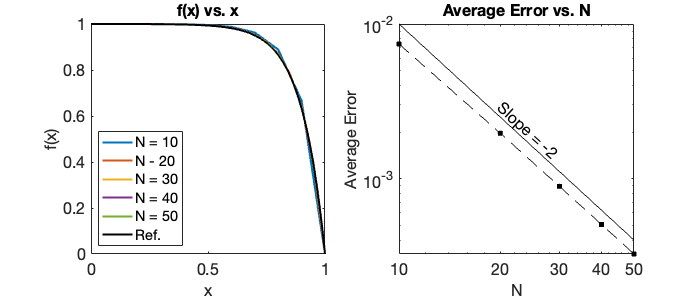
\includegraphics[width=\textwidth]{partA.png}
        \caption{Solution, average error, and runtime for $N = 10, 20, 30, 40, 50$}
        \label{fig:B}
    \end{figure}

    \section*{Part C - Non-linear Problems}
    \Cref{fig:C} shows the solution and pointwise error for the case $U = 0,\ \Gamma = 0.1 + 0.1\varphi$ and $N = 20$ for $Q = 0,\ 0.1,$ and $0.1x$.
    The solution for $Q = 0.1x$ lies between the solutions for $Q = 0$ and $Q = 0.1$.
    This is because the total source flux, given by $Q = \int_{0}^L Q\mathrm{d}l$, satisfies $Q_0 < Q_{0.1x} < Q_{0.1}$ and a larger total source flux results in a higher curve.
    The pointwise error is between the discretized solution and the exact solution is less than the specified tolerance of $1\times 10^{-3}$.
    The iterative solve is what differentiates the approach for solving this nonlinear problem from the approach to solving the linear equation.
    Since the coefficients depend on the solution, an initial guess for the solution must be made and iterated on until a specified convergence tolerance has been met.
    The runtime on a single Apple M2 core for each $Q$, averaged over $1\times 10^6$ runs is given in \cref{tab:c}.
    This runtime is 5.3 times longer than the linear solve for the $N = 20$ case.
    The increase in runtime is because 5 iterations are required to reach convergence and each iteration requires the additional calculation of an error estimate.
    \begin{figure}[h]
        \centering
        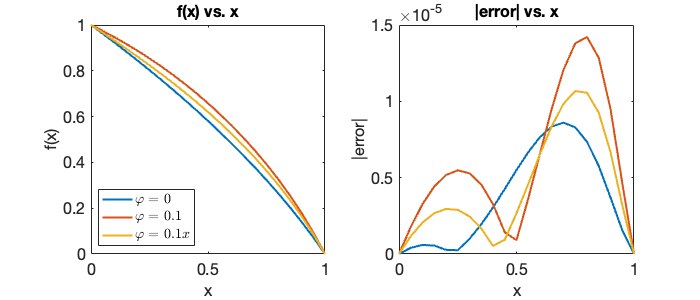
\includegraphics[width=0.66\textwidth]{partC.png}
        \caption{Solution and pointwise error for $Q = 0, 0.1, 0.1x$}
        \label{fig:B}
    \end{figure}
    \begin{table}[h]
        \centering
        \caption{Run time for $Q = 0, 0.1, 0.1x$}
        \begin{tabular}{r | c c c}
            $Q$ & 0 & 0.1 & 0.1x \\ \hline
             Runtime ($\mu$s) & 6.3 & 6.3 & 6.2
        \end{tabular}
        \label{tab:c}
    \end{table}

\end{document}

